\documentclass[12pt, a4paper, oneside]{article}
\usepackage{amsmath, amsthm, amssymb, bm, graphicx, hyperref, mathrsfs, tikz, booktabs, color}

\title{\textbf{Assignment\#6 CS201 Fall 2023}}
\author{Ben Chen(12212231)}
\date{\today}
\linespread{1.5}
\newcounter{problemname}
\newenvironment{problem}{\stepcounter{problemname}\par\noindent\textsc{Problem \arabic{problemname}. }}{\\\par}
\newenvironment{solution}{\par\noindent\textsc{Solution. }}{\\\par}
\newenvironment{note}{\par\noindent\textsc{Note of Problem \arabic{problemname}. }}{\\\par}

\begin{document}

\maketitle

\begin{problem}
    Let $G$ be a simple graph with n vertices.
\end{problem}

\begin{solution}
    \textbf{a)} The maximum number of edges in $G$ is \[ \binom{n}{2} = \frac{n(n-1)}{2} \]
    since each vertex can connect to all other vertices except itself. And the minimum number of edges in $G$ is 0
    since the vertices may be isolated and there is no edge in $G$.
    \newline\textbf{b)} The maximum degrees of vertex in $G$ is $n-1$ since each vertex can connect to all other
    vertices except itself. And the minimum degrees of vertex in $G$ is $0$ since there may be some isolated vertices.
    \newline\textbf{c)} Since the minimum degrees of vertices in $G$ is $(n-1)/2$, suppose a vertex $v$ has degree
    $(n-1)/2$, pick it out and there are $(n-1)$ vertices left. So half of the rest vertices must connect to $v$ which
    gives a connected subgraphs with $(n+1)/2$ vertices, named $G_1$ and the other half of vertices form the other graph
    with $(n-1)/2$ vertices, named $G_2$. The worst case is that $G_1$ and $G_2$ is a complete graph. Consider that, in $G_2$,
    each vertex has degree $(n-3)/2$ which is less than $(n-1)/2$, so there must be a edge between $G_1$ and $G_2$.
    Otherwise, if either $G_1$ or $G_2$ is not a complete graph, there must be a vertex $u$ in $G_1$ or $G_2$ that connects them.
    Therefore, the subgraphs $G_1$ and $G_2$ are connected to each other and $G$ is connected.
\end{solution}

\begin{problem}
    The complementary graph of a graph $G$ is the graph $\overline{G}$ with the same vertices as $G$ and that two vertices in $\overline{G}$ are adjacent if and only if they are not adjacent in $G$.
\end{problem}

\begin{solution}
    \textbf{a)} $\overline{K_n}$ is a graph with $n$ vertices and no edges.
    \newline\textbf{b)} $\overline{K_{m,n}}$ is two complete subgraphs with $m$ and $n$ vertices respectively and they are isolated to each other.
    \newline\textbf{c)} $\overline{C_n}$ has vertices whose degrees are $n-3$ without loops.
    \newline\textbf{d)} $\overline{Q_n}$ has vertices whose degrees are $2^n - 1 - n$ without loops.
\end{solution}

\begin{problem}
    Suppose that there are four employees in the computer support group, and each employees will be assigned to support
    one of four different areas: hardware, software, networking, and wireless. Now Ping is qualified to support hardware
    , networking and wireless; Quiggley is qualified to support software and networking; Ravi is qualified to support networking
    and wireless; Sitea is qualified to support hardware and software.
\end{problem}

\begin{solution}
    \textbf{a)} The bipartie graph is
    \begin{figure*}[!htbp]
        \centering
        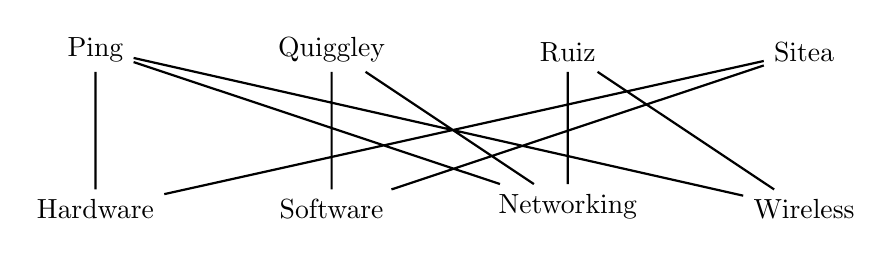
\begin{tikzpicture}[thick]
            \draw (0,0) node[above] (ping) {Ping};
            \draw (3,0) node[above] (quig) {Quiggley};
            \draw (6,0) node[above] (ruiz) {Ruiz};
            \draw (9,0) node[above] (site) {Sitea};
            \draw (0,-2) node[above] (hard) {Hardware};
            \draw (3,-2) node[above] (soft) {Software};
            \draw (6,-2) node[above] (netw) {Networking};
            \draw (9,-2) node[above] (wire) {Wireless};
            \draw (ping) -- (hard)
                  (ping) -- (netw)
                  (ping) -- (wire)
                  (quig) -- (soft)
                  (quig) -- (netw)
                  (ruiz) -- (netw)
                  (ruiz) -- (wire)
                  (site) -- (hard)
                  (site) -- (soft);
        \end{tikzpicture}
    \end{figure*}
    \newline\textbf{b)} The subsets of employees and their neighbors are shown below,
    and it is obvious that the size of neighbors is over than size of employees\newline
    \begin{table}[!htbp]
        \centering
        \begin{tabular}{cc}
            \toprule
            Employees & Neighbors \\\midrule
            Ping & Hardware, Networking, Wireless \\
            Quiggley & Software, Networking \\
            Ruiz & Networking, Wireless \\
            Sitea & Hardware, Software \\
            Ping, Quiggley & Hardware, Software, Networking, Wireless \\
            Ping, Ruiz & Networking, Networking, Wireless \\
            Ping, Sitea & Hardware, Software, Networking, Wireless \\
            Quiggley, Ruiz & Software, Networking, Wireless \\
            Quiggley, Sitea & Hardware, Software, Networking\\
            Ruiz, Sitea & Hardware, Software, Networking, Wireless \\
            Ping, Quiggley, Ruiz & Hardware, Software, Networking, Wireless \\
            Ping, Quiggley, Sitea & Hardware, Software, Networking, Wireless \\
            Ping, Ruiz, Sitea & Hardware, Software, Networking, Wireless \\
            Quiggley, Ruiz, Sitea & Hardware, Software, Networking, Wireless \\
            Ping, Quiggley, Ruiz, Sitea & Hardware, Software, Networking, Wireless \\
            \bottomrule
        \end{tabular}
    \end{table}
    \newline and one of the possible assignment is
    \begin{figure*}[!htbp]
        \centering
        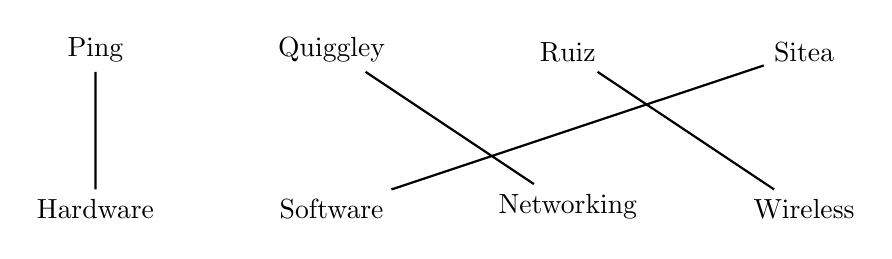
\begin{tikzpicture}[thick]
            \draw (0,0) node[above] (ping) {Ping};
            \draw (3,0) node[above] (quig) {Quiggley};
            \draw (6,0) node[above] (ruiz) {Ruiz};
            \draw (9,0) node[above] (site) {Sitea};
            \draw (0,-2) node[above] (hard) {Hardware};
            \draw (3,-2) node[above] (soft) {Software};
            \draw (6,-2) node[above] (netw) {Networking};
            \draw (9,-2) node[above] (wire) {Wireless};
            \draw (ping) -- (hard)
                  (quig) -- (netw)
                  (ruiz) -- (wire)
                  (site) -- (soft);
        \end{tikzpicture}
    \end{figure*}
\end{solution}

\begin{problem}
    A simple graph $G$ is called self-complementary if $G$ and $\overline{G}$ are isomorphic.
    Show that if $G$ is self-complementary graph with $v$ vertices, then $v\equiv 0\ \text{or}\ 1\ (\text{mod}\ 4)$.
\end{problem}

\begin{solution}
    Since $G$ and $\overline{G}$ are isomorphic, they have the same number of edges. And when we union $G$ and $\overline{G}$,
    we will obtain a complete graph. So the edges of $G$ and $\overline{G}$ are
    \[ \frac{v(v-1)}{4} \]
    So $v$ must be $4k$ or $4k+1$ which gives $v\equiv 0\ \text{or}\ 1\ (\text{mod}\ 4)$.
\end{solution}

\begin{problem}
    Let $G$ be a connected graph. The distance between two vertices $u$ and $v$ in $G$, denoted by $dist(u,v)$, is the
    minimum length of a path between $u$ and $v$. Show that $dist(u,v)$ is a metric on the vertex set of $G$.
\end{problem}

\begin{solution}
    \textbf{a)} Firstly, we shall prove the ``if'' part. Suppose we have $u = v$, than the shortest path is that
    \[ x_0 = x_{n} = u \]
    and there is no edge connect them, so $dist(u,v) = 0$. For the ``only if'' part, we have $dist(u,v) = 0$,
    and suppose $u$ and $v$ are two distinct nodes, then there must be a shortest path
    \[ x_0 = u, x_{n} = v \]
    and there is no edge connect them but $G$ is connected, so by contradictory, $u$ and $v$ must be the same node.
    Since $G$ is connected, there must be a path between $u$ and $v$, so $dist(u,v) \ge 1$ if $u \neq v$.
    \[ \begin{cases}
        dist(u,v) \ge 1, & u\neq v \\
        dist(u,v) = 0, & u = v
    \end{cases} \Rightarrow \forall u,v\in V. \ \ dist(u,v)\ge 0 \]
    \newline\textbf{b)} Suppose the shortest path between $u$ and $v$ is
    \[ e_1, e_2, \cdots, e_n \]
    and the vertices on the path are
    \[ x_0 = u, x_1, x_2, \cdots, x_{n-1}, x_n = v \]
    then (one of) the shortest path between $v$ and $u$ is
    \[ e_n, e_{n-1}, \cdots, e_1 \]
    and the vertices on the path are
    \[ x_0 = v, x_n, x_{n-1}, \cdots, x_1, x_n = u \]
    since edges in $G$ is undirected. So $dist(u,v) = dist(v,u)$.
    \newline\textbf{c)} Suppose that
    \[ dist(u,v) = n > dist(u,w) + dist(w,v) = m \]
    the shortest path between $u$ and $v$ is
    \[ e_1, e_2, \cdots, e_n \]
    the shortest path between $u$ and $w$ is
    \[ e_1, e_2, \cdots, e_k = P_1 \]
    and the shortest path between $w$ and $v$ is
    \[ e_{k+1}, e_{k+2}, \cdots, e_m = P_2\]
    then the shortest path between $u$ and $v$ is
    \[ P_1\cup P_2 =  e_1, e_2, \cdots, e_k, e_{k+1}, e_{k+2}, \cdots, e_m \]
    which means that $dist(u,v) = m \neq n$, by contradictory, we have
    \[ dist(u,v) \le dist(u,w) + dist(w,v) \]
\end{solution}

\begin{problem}
    In an $n$-player round-robin every pair of distinct players compete in a single
    game. Assume that every game has a winner, there are no ties. The results of such a tournament
    can then be represented with a tournament directed graph where the vertices correspond to players
    and there is an edge $x\rightarrow y$ if and only if $x$ beats $y$ in their game.
\end{problem}

\begin{solution}
    \textbf{a)} There is no self loop (i.e. cycle of length 1) in the tournament directed graph since one cannot beat himself. And
    there's no cycle of length 2 since $x$ and $y$ have only one game and one of them must win. So there is only one directed edge
    between $x$ and $y$, $x\rightarrow y$ or $y\rightarrow x$ and not both. So there is no cycle of length 2.
    \newline\textbf{b)} always: antisymmetric and irreflexive\newline
    sometimes: transitive\newline
    never: reflexive and symmetric
    \newline\textbf{c)} As mentioned previously, the tournament directed graph is antisymmetric and irreflexive, since there is no self loop
    and there is no cycle of length 2. And the each pair of player is comparable since there must be only one directed edge between them. So
    we shall prove the transitive property. Suppose that $x\rightarrow y$ and $y\rightarrow z$, which is $x$ beats $y$ and $y$ beats $z$, so $x$ beats $z$,
    then there is a directed edge $x\rightarrow z$ which makes no circle of length 3. So the only if part is proved. And for the if part, suppose that
    there is no circle of length 3 and $x$ beats $y$ and $y$ beats $z$, then $z$ beats $x$ cannot hold. On the contrary, $x$ beats $z$ definitely holds since
    there must be a directed edge between $x$ and $z$. Therefore, the tournament graph is transitive iff there is no circle of length 3, and the strict
    total order holds.
\end{solution}

\begin{problem}
    Let $G$ be a connected simple graph. Show that if an edge in a connected graph is not contained in any simple circuit,
    then this edge is a cut edge.
\end{problem}

\begin{solution}
    Suppose $e = (u,v)$ is not a cut edge, then by definition, the removal of it will not cause the graph disconnected
    so there exists a path between $u$ and $v$ after the removal of $e$ since $G$ is connected. So adding $e$ to the path
    will form a simple circuit which contains $e$, which gives that $e$ is contained in a simple circuit. By contradictory,
    $e$ is a cut edge if it is not contained in any simple circuit.
\end{solution}

\begin{problem}
    Given a graph $G$, its line graph $L(G)$ is the graph whose vertices are the edges of $G$ and two vertices of $L(G)$
    are adjacent if and only if the corresponding edges of $G$ are incident with the same vertex. Prove that if $G$ is
    regular, then $L(G)$ has an euler circuit.
\end{problem}

\begin{solution}
    Since $G$ is connected, for any two vertices $u$ and $v$ in $G$, there is a path between them
    \[ e_1, e_2, \cdots, e_n \]
    and the vertices on the path are
    \[ x_0 = u, x_1, x_2, \cdots, x_{n-1}, x_n = v \]
    so in the line graph $L(G)$, there is a path between $e_1$ and $e_n$, which is
    \[ x_1, x_2, \cdots, x_{n-1}\]
    so $L(G)$ is connected. The degree of vertices in $L(G)$ is $2k - 2$ where $k$ is the degree of vertices in $G$
    since the edge in $G$ has two vertices whose degrees are both $k$, so the corresponding vertex in $L(G)$ has $2(k-2)$ edges.
    So the degree of vertices in $L(G)$ is even. The above condition gives that $L(G)$ has an euler circuit.
\end{solution}

\begin{problem}
    Prove that every $n$-cube $Q_n$ has a hamiltonian circuit.
\end{problem}

\begin{solution}
    \textbf{Base Step:} For $n = 1$, it holds trivially.
    \newline\textbf{Inductive Step:} For $n = k$, suppose that $Q_k$ has a hamiltonian circuit, then for $n = k+1$ we have
    \[ Q_{n+1} = Q_{n} \cup Q^{\prime}_{n} \cup E \]
    where $E$ is the set of edges that connect the corresponding vertices in $Q_{n}$ and $Q^{\prime}_{n}$.
    Suppose the hamilton circuit in $Q_{n}$ is
    \[ x_0, x_1, \cdots, x_{2^n-1}, x_0 \]
    and the hamilton circuit in $Q^{\prime}_{n}$ is
    \[ x^{\prime}_0, x^{\prime}_1, \cdots, x^{\prime}_{2^n-1}, x^{\prime}_0 \]
    then we can construct a hamilton circuit in $Q_{n+1}$ as follows
    \[ x_0, x_1, \cdots, x_{2^n-1}, x^{\prime}_{2^n-1}, x^{\prime}_{2^n-2}, \cdots, x^{\prime}_1, x^{\prime}_0, x_0 \]
    which passes the edges exactly once. So $Q_{n+1}$ has a hamilton circuit. Therefore, by induction,
    every $n$-cube $Q_n$ has a hamiltonian circuit.
\end{solution}

\begin{problem}
    Show that if $G$ is simple graph with at least 11 vertices, then $G$ or $\overline{G}$ is not planar.
\end{problem}

\begin{solution}
    For a simple graph $G$ with $n$ vertices and $m$ edges, its complement has
    \[ \frac{n(n-1)}{2} - m \]
    edges. Suppose that $G$ and $\overline{G}$ is planar, then by Euler's formula, we have
    \[ m \le 3n - 6\]
    and
    \[ \frac{n(n-1)}{2} - m \le 3n - 6 \]
    by solving the inequality, we have
    \[ n \le 10 \]
    so by contradictory, if $G$ is simple graph with at least 11 vertices, then $G$ or $\overline{G}$ is not planar.
\end{solution}

\begin{problem}
    Suppose that a connected planar simple graph with $e$ edges and $v$ vertices contains no simple circuits of length 4
    or less. Show that $e\le (5/3)v - (10/3)$ if $v\ge 4$.
\end{problem}

\begin{solution}
    Since the graph contains no circuirs of length 4 or less, every region has at least 5 edges. So
    \[ 2e = \sum_{R} \deg(R) \ge 5r \]
    where $r$ is the number of regions. Since $G$ is planar, from the Euler's formula, we have
    \[ r = e - v + 2 \ge \frac{2}{5} e \]
    so
    \[ e\le \frac{5}{3}v - \frac{10}{3} \]
\end{solution}

\begin{problem}
    There are 17 students who communicates with each other discussing problems in discrete math. There are 3 possible problems
    and each pair of studnets discuss one of them. Prove that there are at least 3 students who are all pairwise discussing the
    same problem.
\end{problem}

\begin{solution}
    The graph of the students is a complete simple graph with 17 vertices and the edges represent the communication between students.
    And we assign a color to each edge which represents the problem they are discussing. So there are 3 colors in total. Suppose that
    there is a student $S$ who has 16 edges with three colors, denotes by
    \[ SS_1, SS_2, \cdots, SS_{16} \]
    from the Pigeonhole Principle, there must be at least 6 edges with the same color $C_1$, suppose that they are
    \[ SS_1, SS_2, \cdots, SS_6 \]
    then consider the edges between $S_1, S_2, \cdots, S_6$, if there is an edge with the same color $C_1$, then we have 3 students who are
    all pairwise discussing the same problem. Otherwise, consider the edges from $S_1$ to $S_2, S_3, \cdots, S_6$, also from the Pigeonhole
    Principle, there must be at least 3 edges with the same color $C_2$, suppose that they are
    \[ S_1S_2, S_1S_3, S_1S_4 \]
    if one of edges of $S_2S_3S_4$ is the same color $C_2$, then we have 3 students who are all pairwise discussing the same problem. Otherwise,
    the edges $S_2S_3, S_3S_4, S_2S_4$ are in the same color $C_3$.
\end{solution}

\begin{problem}
    The rooted Fibonacci trees $T_n$ are defined recursively as follows: $T_1$ and $T_2$ are both the rooted trees consisting
    of a simgle vertex, and for $n>3$, the rooted tree $T_n$ is constructed from a root with $T_{n-1}$ as its left subtree and
    $T_{n-2}$ as its right subtree.
\end{problem}

\begin{solution}
    \textbf{a)} The number of vertices of $T_n$ are
    \[ V(n) = V(n-1) + V(n-2) + 1 \]
    where $V(n)$ is the number of vertices of $T_n$, solving the nonhomogeneous linear recurrence relation, we have
    \[ V(n) = \frac{2}{\sqrt{5}}\left( \left( \frac{1 + \sqrt{5}}{2}\right)^{n+1} - \left(\frac{1 - \sqrt{5}}{2}\right)^{n+1} \right) - 1 \]
    And it is obvious that the Fibonacci trees are complete binary trees, so the number of leaves of $T_n$ is $2^{n - 1}$ and the number of
    internal vertices is 
    \[ V(n) - 2^{n-2} \] \[ = \frac{2}{\sqrt{5}}\left( \left( \frac{1 + \sqrt{5}}{2}\right)^{n+1} - \left(\frac{1 - \sqrt{5}}{2}\right)^{n+1} \right) - 2^{n - 2} - 1 \]
    for $n > 2$. Otherwise the number of internal vertices is 1 and number of leaves is 0 since there is one root vertex.
    \newline\textbf{b)} The height of $T_n$ is $n - 1$, since for the left subtrees
    \[H(n) = H(n-1) + 1, \quad n > 2 \]
    where $H(n)$ is the height of $T_n$ and $H_1 = H_2 = 1$. And for the right subtrees, since height of $T(n-2)$ is less than or equal to the height of $T(n-1)$,
    the height is mainly decided by the left subtrees.
\end{solution}

\begin{problem}
    Calculate the value of the postfix expression ``3 2 * 2 $\uparrow$ 5 3 - 8 4 / * -'' and show the steps.
\end{problem}

\begin{solution}
    We can build a binary tree from the postfix expression, and the value of the expression is the result of the root of the tree
    \begin{figure}[!htbp]
        \centering
        \begin{tikzpicture}[
                level distance=2cm,
                level 1/.style={sibling distance=5cm},
                level 2/.style={sibling distance=3cm},
                level 3/.style={sibling distance=1.5cm}
            ]
            \node {$-\ (32)$}
            child { 
                node {$\uparrow\ (36)$}
                child { 
                    node {$*\ (6)$}
                    child {node {3}}
                    child {node {2}}
                }
                child { node {2} }
            }
            child {
                node {$*\ (6)$}
                child {
                    node {$-\ (2)$}
                    child { node {5} }
                    child { node {3} }
                }
                child {
                    node {$/\ (2)$}
                    child { node {8} }
                    child { node {4} }
                }
            };
        \end{tikzpicture}
    \end{figure}
    \newline The result of the expression is 32.
\end{solution}

\begin{problem}
    Consider the graph shown below and answer the following questions.
\end{problem}

\begin{solution}
    \textbf{a)} The first step is to add vertex $a$ to the set. Then, choose a vertex $u$ that is currently the closest to $a$ (i.e. $L(u)$ is the smallest),
    to add to the set and iterate all the vertices of the graph that is not in the set, update the $L(u)$. Keep doing the second step until
    the destination vertex $f$ is added to the set. The following graphs show the whole process.
    \begin{figure*}[!htbp]
        \centering
        \begin{minipage}[t]{0.48\textwidth}
            \centering
            \caption{(a)}
            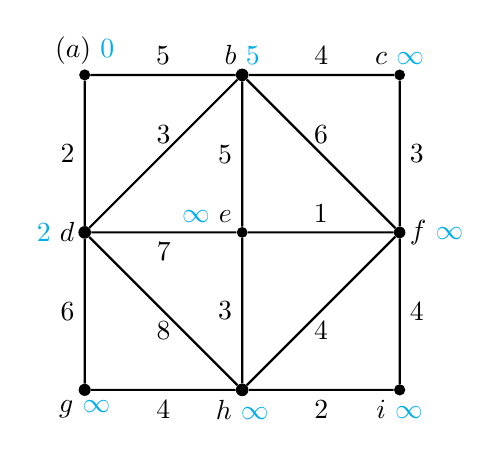
\begin{tikzpicture}[thick]
            \draw (0,0)  node[circle,fill=black,scale=0.25] (a) {a};
            \draw (2,0)  node[circle,fill=black,scale=0.25] (b) {b};
            \draw (4,0)  node[circle,fill=black,scale=0.25] (c) {c};
            \draw (0,-2) node[circle,fill=black,scale=0.25] (d) {d};
            \draw (2,-2) node[circle,fill=black,scale=0.25] (e) {e};
            \draw (4,-2) node[circle,fill=black,scale=0.25] (f) {f};
            \draw (0,-4) node[circle,fill=black,scale=0.25] (g) {g};
            \draw (2,-4) node[circle,fill=black,scale=0.25] (h) {h};
            \draw (4,-4) node[circle,fill=black,scale=0.25] (i) {i};
            \node[above] at (0,0) {$(a)$ \textcolor{cyan}{$0$}};
            \node[above] at (2,0) {$b$ \textcolor{cyan}{$5$}};
            \node[above] at (4,0) {$c$ \textcolor{cyan}{$\infty$}};
            \node[left] at (0,-2) {\textcolor{cyan}{$2$} $d$};
            \node[above left] at (2,-2) {\textcolor{cyan}{$\infty$} $e$};
            \node[right] at (4,-2) {$f$ \textcolor{cyan}{$\infty$}};
            \node[below] at (0,-4) {$g$ \textcolor{cyan}{$\infty$}};
            \node[below] at (2,-4) {$h$ \textcolor{cyan}{$\infty$}};
            \node[below] at (4,-4) {$i$ \textcolor{cyan}{$\infty$}};
            \draw (a) -- (b) node [midway, above] {5}
                  (a) -- (d) node [midway, left] {2}
                  (b) -- (d) node [midway, above] {3}
                  (b) -- (c) node [midway, above] {4}
                  (b) -- (f) node [midway, above] {6}
                  (b) -- (e) node [midway, left] {5}
                  (c) -- (f) node [midway, right] {3}
                  (d) -- (e) node [midway, below] {7}
                  (d) -- (g) node [midway, left] {6}
                  (d) -- (h) node [midway, below] {8}
                  (e) -- (f) node [midway, above] {1}
                  (e) -- (h) node [midway, left] {3}
                  (f) -- (h) node [midway, below] {4}
                  (f) -- (i) node [midway, right] {4}
                  (g) -- (h) node [midway, below] {4}
                  (h) -- (i) node [midway, below] {2};
        \end{tikzpicture}
    \end{minipage}
    \begin{minipage}[t]{0.48\textwidth}
        \centering
        \caption{(b)}
        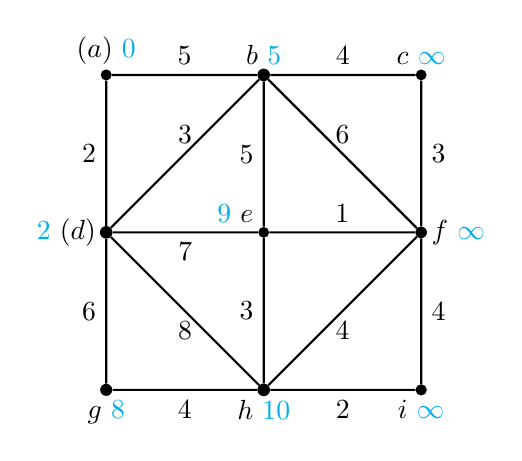
\begin{tikzpicture}[thick]
            \draw (0,0)  node[circle,fill=black,scale=0.25] (a) {a};
            \draw (2,0)  node[circle,fill=black,scale=0.25] (b) {b};
            \draw (4,0)  node[circle,fill=black,scale=0.25] (c) {c};
            \draw (0,-2) node[circle,fill=black,scale=0.25] (d) {d};
            \draw (2,-2) node[circle,fill=black,scale=0.25] (e) {e};
            \draw (4,-2) node[circle,fill=black,scale=0.25] (f) {f};
            \draw (0,-4) node[circle,fill=black,scale=0.25] (g) {g};
            \draw (2,-4) node[circle,fill=black,scale=0.25] (h) {h};
            \draw (4,-4) node[circle,fill=black,scale=0.25] (i) {i};
            \node[above] at (0,0) {$(a)$ \textcolor{cyan}{$0$}};
            \node[above] at (2,0) {$b$ \textcolor{cyan}{$5$}};
            \node[above] at (4,0) {$c$ \textcolor{cyan}{$\infty$}};
            \node[left] at (0,-2) {\textcolor{cyan}{$2$} $(d)$};
            \node[above left] at (2,-2) {\textcolor{cyan}{$9$} $e$};
            \node[right] at (4,-2) {$f$ \textcolor{cyan}{$\infty$}};
            \node[below] at (0,-4) {$g$ \textcolor{cyan}{$8$}};
            \node[below] at (2,-4) {$h$ \textcolor{cyan}{$10$}};
            \node[below] at (4,-4) {$i$ \textcolor{cyan}{$\infty$}};
            \draw (a) -- (b) node [midway, above] {5}
                  (a) -- (d) node [midway, left] {2}
                  (b) -- (d) node [midway, above] {3}
                  (b) -- (c) node [midway, above] {4}
                  (b) -- (f) node [midway, above] {6}
                  (b) -- (e) node [midway, left] {5}
                  (c) -- (f) node [midway, right] {3}
                  (d) -- (e) node [midway, below] {7}
                  (d) -- (g) node [midway, left] {6}
                  (d) -- (h) node [midway, below] {8}
                  (e) -- (f) node [midway, above] {1}
                  (e) -- (h) node [midway, left] {3}
                  (f) -- (h) node [midway, below] {4}
                  (f) -- (i) node [midway, right] {4}
                  (g) -- (h) node [midway, below] {4}
                  (h) -- (i) node [midway, below] {2};
    \end{tikzpicture}
    \end{minipage}
    \begin{minipage}[t]{0.48\textwidth}
    \centering
    \caption{(c)}
    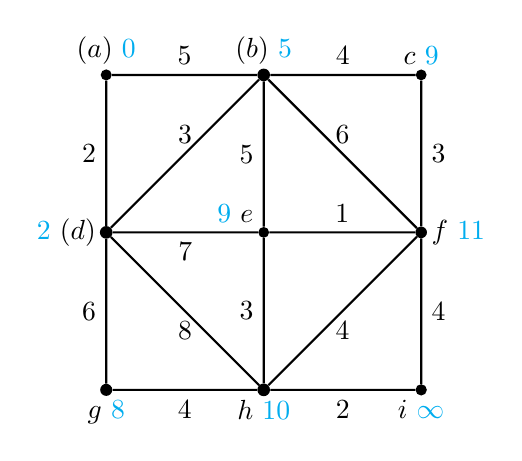
\begin{tikzpicture}[thick]
        \draw (0,0)  node[circle,fill=black,scale=0.25] (a) {a};
        \draw (2,0)  node[circle,fill=black,scale=0.25] (b) {b};
        \draw (4,0)  node[circle,fill=black,scale=0.25] (c) {c};
        \draw (0,-2) node[circle,fill=black,scale=0.25] (d) {d};
        \draw (2,-2) node[circle,fill=black,scale=0.25] (e) {e};
        \draw (4,-2) node[circle,fill=black,scale=0.25] (f) {f};
        \draw (0,-4) node[circle,fill=black,scale=0.25] (g) {g};
        \draw (2,-4) node[circle,fill=black,scale=0.25] (h) {h};
        \draw (4,-4) node[circle,fill=black,scale=0.25] (i) {i};
        \node[above] at (0,0) {$(a)$ \textcolor{cyan}{$0$}};
        \node[above] at (2,0) {$(b)$ \textcolor{cyan}{$5$}};
        \node[above] at (4,0) {$c$ \textcolor{cyan}{$9$}};
        \node[left] at (0,-2) {\textcolor{cyan}{$2$} $(d)$};
        \node[above left] at (2,-2) {\textcolor{cyan}{$9$} $e$};
        \node[right] at (4,-2) {$f$ \textcolor{cyan}{$11$}};
        \node[below] at (0,-4) {$g$ \textcolor{cyan}{$8$}};
        \node[below] at (2,-4) {$h$ \textcolor{cyan}{$10$}};
        \node[below] at (4,-4) {$i$ \textcolor{cyan}{$\infty$}};
        \draw (a) -- (b) node [midway, above] {5}
              (a) -- (d) node [midway, left] {2}
              (b) -- (d) node [midway, above] {3}
              (b) -- (c) node [midway, above] {4}
              (b) -- (f) node [midway, above] {6}
              (b) -- (e) node [midway, left] {5}
              (c) -- (f) node [midway, right] {3}
              (d) -- (e) node [midway, below] {7}
              (d) -- (g) node [midway, left] {6}
              (d) -- (h) node [midway, below] {8}
              (e) -- (f) node [midway, above] {1}
              (e) -- (h) node [midway, left] {3}
              (f) -- (h) node [midway, below] {4}
              (f) -- (i) node [midway, right] {4}
              (g) -- (h) node [midway, below] {4}
              (h) -- (i) node [midway, below] {2};
    \end{tikzpicture}
    \end{minipage}
    \begin{minipage}[t]{0.48\textwidth}
        \centering
        \caption{(d)}
    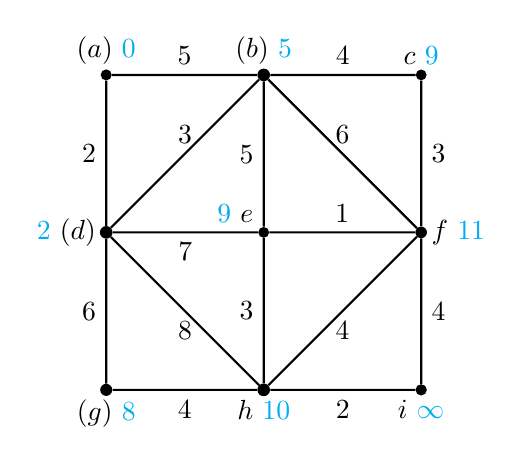
\begin{tikzpicture}[thick]
        \draw (0,0)  node[circle,fill=black,scale=0.25] (a) {a};
        \draw (2,0)  node[circle,fill=black,scale=0.25] (b) {b};
        \draw (4,0)  node[circle,fill=black,scale=0.25] (c) {c};
        \draw (0,-2) node[circle,fill=black,scale=0.25] (d) {d};
        \draw (2,-2) node[circle,fill=black,scale=0.25] (e) {e};
        \draw (4,-2) node[circle,fill=black,scale=0.25] (f) {f};
        \draw (0,-4) node[circle,fill=black,scale=0.25] (g) {g};
        \draw (2,-4) node[circle,fill=black,scale=0.25] (h) {h};
        \draw (4,-4) node[circle,fill=black,scale=0.25] (i) {i};
        \node[above] at (0,0) {$(a)$ \textcolor{cyan}{$0$}};
        \node[above] at (2,0) {$(b)$ \textcolor{cyan}{$5$}};
        \node[above] at (4,0) {$c$ \textcolor{cyan}{$9$}};
        \node[left] at (0,-2) {\textcolor{cyan}{$2$} $(d)$};
        \node[above left] at (2,-2) {\textcolor{cyan}{$9$} $e$};
        \node[right] at (4,-2) {$f$ \textcolor{cyan}{$11$}};
        \node[below] at (0,-4) {$(g)$ \textcolor{cyan}{$8$}};
        \node[below] at (2,-4) {$h$ \textcolor{cyan}{$10$}};
        \node[below] at (4,-4) {$i$ \textcolor{cyan}{$\infty$}};
        \draw (a) -- (b) node [midway, above] {5}
              (a) -- (d) node [midway, left] {2}
              (b) -- (d) node [midway, above] {3}
              (b) -- (c) node [midway, above] {4}
              (b) -- (f) node [midway, above] {6}
              (b) -- (e) node [midway, left] {5}
              (c) -- (f) node [midway, right] {3}
              (d) -- (e) node [midway, below] {7}
              (d) -- (g) node [midway, left] {6}
              (d) -- (h) node [midway, below] {8}
              (e) -- (f) node [midway, above] {1}
              (e) -- (h) node [midway, left] {3}
              (f) -- (h) node [midway, below] {4}
              (f) -- (i) node [midway, right] {4}
              (g) -- (h) node [midway, below] {4}
              (h) -- (i) node [midway, below] {2};
    \end{tikzpicture}
    \end{minipage}
    \begin{minipage}[t]{0.48\textwidth}
        \centering
        \caption{(e)}
    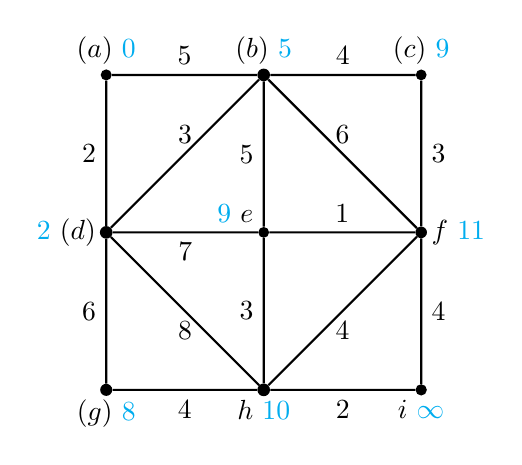
\begin{tikzpicture}[thick]
        \draw (0,0)  node[circle,fill=black,scale=0.25] (a) {a};
        \draw (2,0)  node[circle,fill=black,scale=0.25] (b) {b};
        \draw (4,0)  node[circle,fill=black,scale=0.25] (c) {c};
        \draw (0,-2) node[circle,fill=black,scale=0.25] (d) {d};
        \draw (2,-2) node[circle,fill=black,scale=0.25] (e) {e};
        \draw (4,-2) node[circle,fill=black,scale=0.25] (f) {f};
        \draw (0,-4) node[circle,fill=black,scale=0.25] (g) {g};
        \draw (2,-4) node[circle,fill=black,scale=0.25] (h) {h};
        \draw (4,-4) node[circle,fill=black,scale=0.25] (i) {i};
        \node[above] at (0,0) {$(a)$ \textcolor{cyan}{$0$}};
        \node[above] at (2,0) {$(b)$ \textcolor{cyan}{$5$}};
        \node[above] at (4,0) {$(c)$ \textcolor{cyan}{$9$}};
        \node[left] at (0,-2) {\textcolor{cyan}{$2$} $(d)$};
        \node[above left] at (2,-2) {\textcolor{cyan}{$9$} $e$};
        \node[right] at (4,-2) {$f$ \textcolor{cyan}{$11$}};
        \node[below] at (0,-4) {$(g)$ \textcolor{cyan}{$8$}};
        \node[below] at (2,-4) {$h$ \textcolor{cyan}{$10$}};
        \node[below] at (4,-4) {$i$ \textcolor{cyan}{$\infty$}};
        \draw (a) -- (b) node [midway, above] {5}
              (a) -- (d) node [midway, left] {2}
              (b) -- (d) node [midway, above] {3}
              (b) -- (c) node [midway, above] {4}
              (b) -- (f) node [midway, above] {6}
              (b) -- (e) node [midway, left] {5}
              (c) -- (f) node [midway, right] {3}
              (d) -- (e) node [midway, below] {7}
              (d) -- (g) node [midway, left] {6}
              (d) -- (h) node [midway, below] {8}
              (e) -- (f) node [midway, above] {1}
              (e) -- (h) node [midway, left] {3}
              (f) -- (h) node [midway, below] {4}
              (f) -- (i) node [midway, right] {4}
              (g) -- (h) node [midway, below] {4}
              (h) -- (i) node [midway, below] {2};
    \end{tikzpicture}
    \end{minipage}
    \begin{minipage}[t]{0.48\textwidth}
        \centering
        \caption{(f)}
    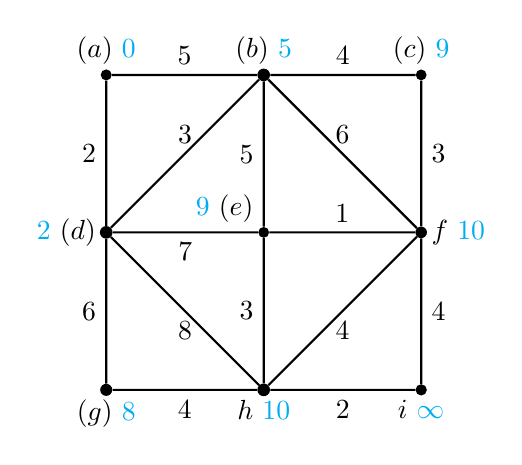
\begin{tikzpicture}[thick]
        \draw (0,0)  node[circle,fill=black,scale=0.25] (a) {a};
        \draw (2,0)  node[circle,fill=black,scale=0.25] (b) {b};
        \draw (4,0)  node[circle,fill=black,scale=0.25] (c) {c};
        \draw (0,-2) node[circle,fill=black,scale=0.25] (d) {d};
        \draw (2,-2) node[circle,fill=black,scale=0.25] (e) {e};
        \draw (4,-2) node[circle,fill=black,scale=0.25] (f) {f};
        \draw (0,-4) node[circle,fill=black,scale=0.25] (g) {g};
        \draw (2,-4) node[circle,fill=black,scale=0.25] (h) {h};
        \draw (4,-4) node[circle,fill=black,scale=0.25] (i) {i};
        \node[above] at (0,0) {$(a)$ \textcolor{cyan}{$0$}};
        \node[above] at (2,0) {$(b)$ \textcolor{cyan}{$5$}};
        \node[above] at (4,0) {$(c)$ \textcolor{cyan}{$9$}};
        \node[left] at (0,-2) {\textcolor{cyan}{$2$} $(d)$};
        \node[above left] at (2,-2) {\textcolor{cyan}{$9$} $(e)$};
        \node[right] at (4,-2) {$f$ \textcolor{cyan}{$10$}};
        \node[below] at (0,-4) {$(g)$ \textcolor{cyan}{$8$}};
        \node[below] at (2,-4) {$h$ \textcolor{cyan}{$10$}};
        \node[below] at (4,-4) {$i$ \textcolor{cyan}{$\infty$}};
        \draw (a) -- (b) node [midway, above] {5}
              (a) -- (d) node [midway, left] {2}
              (b) -- (d) node [midway, above] {3}
              (b) -- (c) node [midway, above] {4}
              (b) -- (f) node [midway, above] {6}
              (b) -- (e) node [midway, left] {5}
              (c) -- (f) node [midway, right] {3}
              (d) -- (e) node [midway, below] {7}
              (d) -- (g) node [midway, left] {6}
              (d) -- (h) node [midway, below] {8}
              (e) -- (f) node [midway, above] {1}
              (e) -- (h) node [midway, left] {3}
              (f) -- (h) node [midway, below] {4}
              (f) -- (i) node [midway, right] {4}
              (g) -- (h) node [midway, below] {4}
              (h) -- (i) node [midway, below] {2};
    \end{tikzpicture}
    \end{minipage}
    \end{figure*}
    So the shortest path is $a \rightarrow d \rightarrow e \rightarrow f$ with length 10.
    \newline\textbf{b)} We can start from the vertex $a$ and get the edge with minimum weight
    \begin{figure*}[!htbp]
        \centering
    \begin{tikzpicture}[thick]
        \draw (0,0)  node[circle,fill=black,scale=0.25] (a) {a};
        \draw (2,0)  node[circle,fill=black,scale=0.25] (b) {b};
        \draw (4,0)  node[circle,fill=black,scale=0.25] (c) {c};
        \draw (0,-2) node[circle,fill=black,scale=0.25] (d) {d};
        \draw (2,-2) node[circle,fill=black,scale=0.25] (e) {e};
        \draw (4,-2) node[circle,fill=black,scale=0.25] (f) {f};
        \draw (0,-4) node[circle,fill=black,scale=0.25] (g) {g};
        \draw (2,-4) node[circle,fill=black,scale=0.25] (h) {h};
        \draw (4,-4) node[circle,fill=black,scale=0.25] (i) {i};
        \node[above] at (0,0) {$a$};
        \node[above] at (2,0) {$b$};
        \node[above] at (4,0) {$c$};
        \node[left] at (0,-2) {$d$};
        \node[above left] at (2,-2) {$e$};
        \node[right] at (4,-2) {$f$};
        \node[below] at (0,-4) {$g$};
        \node[below] at (2,-4) {$h$};
        \node[below] at (4,-4) {$i$};
        \draw (a) -- (d) node [midway, left] {2};
    \end{tikzpicture}
    \end{figure*}
    \newline and keep adding edges with minimum weight, which is $d \rightarrow b$ with weight 3
    \begin{figure*}[!htbp]
        \centering
    \begin{tikzpicture}[thick]
        \draw (0,0)  node[circle,fill=black,scale=0.25] (a) {a};
        \draw (2,0)  node[circle,fill=black,scale=0.25] (b) {b};
        \draw (4,0)  node[circle,fill=black,scale=0.25] (c) {c};
        \draw (0,-2) node[circle,fill=black,scale=0.25] (d) {d};
        \draw (2,-2) node[circle,fill=black,scale=0.25] (e) {e};
        \draw (4,-2) node[circle,fill=black,scale=0.25] (f) {f};
        \draw (0,-4) node[circle,fill=black,scale=0.25] (g) {g};
        \draw (2,-4) node[circle,fill=black,scale=0.25] (h) {h};
        \draw (4,-4) node[circle,fill=black,scale=0.25] (i) {i};
        \node[above] at (0,0) {$a$};
        \node[above] at (2,0) {$b$};
        \node[above] at (4,0) {$c$};
        \node[left] at (0,-2) {$d$};
        \node[above left] at (2,-2) {$e$};
        \node[right] at (4,-2) {$f$};
        \node[below] at (0,-4) {$g$};
        \node[below] at (2,-4) {$h$};
        \node[below] at (4,-4) {$i$};
        \draw (a) -- (d) node [midway, left] {2}
              (b) -- (d) node [midway, above] {3};
    \end{tikzpicture}
    \end{figure*}
    \newline then we add $b \rightarrow c$ with weight 4
    \begin{figure*}[!htbp]
        \centering
    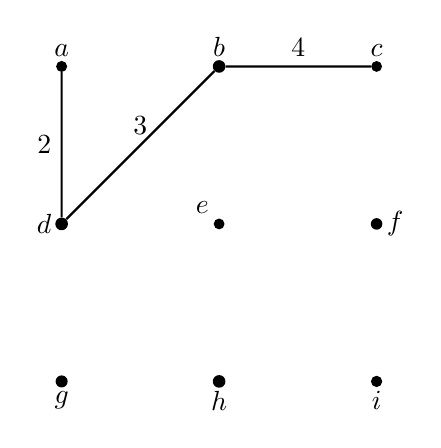
\begin{tikzpicture}[thick]
        \draw (0,0)  node[circle,fill=black,scale=0.25] (a) {a};
        \draw (2,0)  node[circle,fill=black,scale=0.25] (b) {b};
        \draw (4,0)  node[circle,fill=black,scale=0.25] (c) {c};
        \draw (0,-2) node[circle,fill=black,scale=0.25] (d) {d};
        \draw (2,-2) node[circle,fill=black,scale=0.25] (e) {e};
        \draw (4,-2) node[circle,fill=black,scale=0.25] (f) {f};
        \draw (0,-4) node[circle,fill=black,scale=0.25] (g) {g};
        \draw (2,-4) node[circle,fill=black,scale=0.25] (h) {h};
        \draw (4,-4) node[circle,fill=black,scale=0.25] (i) {i};
        \node[above] at (0,0) {$a$};
        \node[above] at (2,0) {$b$};
        \node[above] at (4,0) {$c$};
        \node[left] at (0,-2) {$d$};
        \node[above left] at (2,-2) {$e$};
        \node[right] at (4,-2) {$f$};
        \node[below] at (0,-4) {$g$};
        \node[below] at (2,-4) {$h$};
        \node[below] at (4,-4) {$i$};
        \draw (a) -- (d) node [midway, left] {2}
              (b) -- (d) node [midway, above] {3}
              (b) -- (c) node [midway, above] {4};
    \end{tikzpicture}
    \end{figure*}
    \newline and then $c \rightarrow f$ with weight 3
    \begin{figure*}[!htbp]
        \centering
    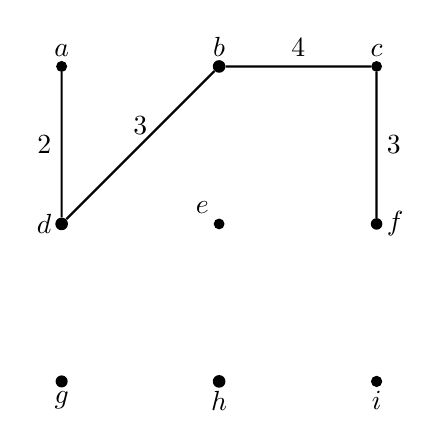
\begin{tikzpicture}[thick]
        \draw (0,0)  node[circle,fill=black,scale=0.25] (a) {a};
        \draw (2,0)  node[circle,fill=black,scale=0.25] (b) {b};
        \draw (4,0)  node[circle,fill=black,scale=0.25] (c) {c};
        \draw (0,-2) node[circle,fill=black,scale=0.25] (d) {d};
        \draw (2,-2) node[circle,fill=black,scale=0.25] (e) {e};
        \draw (4,-2) node[circle,fill=black,scale=0.25] (f) {f};
        \draw (0,-4) node[circle,fill=black,scale=0.25] (g) {g};
        \draw (2,-4) node[circle,fill=black,scale=0.25] (h) {h};
        \draw (4,-4) node[circle,fill=black,scale=0.25] (i) {i};
        \node[above] at (0,0) {$a$};
        \node[above] at (2,0) {$b$};
        \node[above] at (4,0) {$c$};
        \node[left] at (0,-2) {$d$};
        \node[above left] at (2,-2) {$e$};
        \node[right] at (4,-2) {$f$};
        \node[below] at (0,-4) {$g$};
        \node[below] at (2,-4) {$h$};
        \node[below] at (4,-4) {$i$};
        \draw (a) -- (d) node [midway, left] {2}
              (b) -- (d) node [midway, above] {3}
              (b) -- (c) node [midway, above] {4}
              (c) -- (f) node [midway, right] {3};
    \end{tikzpicture}
    \end{figure*}
    \newline and then $f \rightarrow e$ with weight 1
    \begin{figure*}[!htbp]
        \centering
    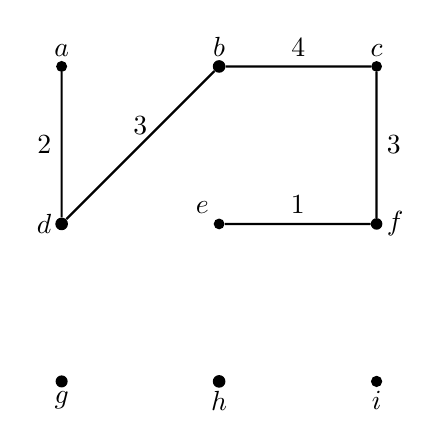
\begin{tikzpicture}[thick]
        \draw (0,0)  node[circle,fill=black,scale=0.25] (a) {a};
        \draw (2,0)  node[circle,fill=black,scale=0.25] (b) {b};
        \draw (4,0)  node[circle,fill=black,scale=0.25] (c) {c};
        \draw (0,-2) node[circle,fill=black,scale=0.25] (d) {d};
        \draw (2,-2) node[circle,fill=black,scale=0.25] (e) {e};
        \draw (4,-2) node[circle,fill=black,scale=0.25] (f) {f};
        \draw (0,-4) node[circle,fill=black,scale=0.25] (g) {g};
        \draw (2,-4) node[circle,fill=black,scale=0.25] (h) {h};
        \draw (4,-4) node[circle,fill=black,scale=0.25] (i) {i};
        \node[above] at (0,0) {$a$};
        \node[above] at (2,0) {$b$};
        \node[above] at (4,0) {$c$};
        \node[left] at (0,-2) {$d$};
        \node[above left] at (2,-2) {$e$};
        \node[right] at (4,-2) {$f$};
        \node[below] at (0,-4) {$g$};
        \node[below] at (2,-4) {$h$};
        \node[below] at (4,-4) {$i$};
        \draw (a) -- (d) node [midway, left] {2}
              (b) -- (d) node [midway, above] {3}
              (b) -- (c) node [midway, above] {4}
              (c) -- (f) node [midway, right] {3}
              (e) -- (f) node [midway, above] {1};
    \end{tikzpicture}
    \end{figure*}
    \newline and then $e \rightarrow h$ with weight 3
    \begin{figure*}[!htbp]
        \centering
    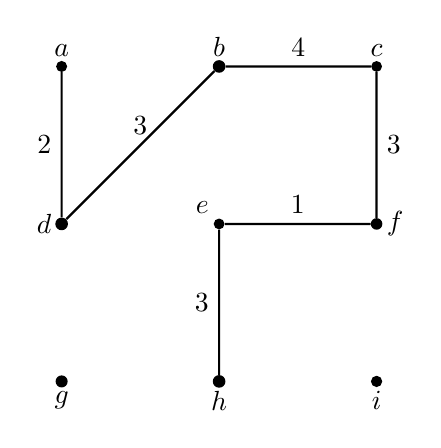
\begin{tikzpicture}[thick]
        \draw (0,0)  node[circle,fill=black,scale=0.25] (a) {a};
        \draw (2,0)  node[circle,fill=black,scale=0.25] (b) {b};
        \draw (4,0)  node[circle,fill=black,scale=0.25] (c) {c};
        \draw (0,-2) node[circle,fill=black,scale=0.25] (d) {d};
        \draw (2,-2) node[circle,fill=black,scale=0.25] (e) {e};
        \draw (4,-2) node[circle,fill=black,scale=0.25] (f) {f};
        \draw (0,-4) node[circle,fill=black,scale=0.25] (g) {g};
        \draw (2,-4) node[circle,fill=black,scale=0.25] (h) {h};
        \draw (4,-4) node[circle,fill=black,scale=0.25] (i) {i};
        \node[above] at (0,0) {$a$};
        \node[above] at (2,0) {$b$};
        \node[above] at (4,0) {$c$};
        \node[left] at (0,-2) {$d$};
        \node[above left] at (2,-2) {$e$};
        \node[right] at (4,-2) {$f$};
        \node[below] at (0,-4) {$g$};
        \node[below] at (2,-4) {$h$};
        \node[below] at (4,-4) {$i$};
        \draw (a) -- (d) node [midway, left] {2}
              (b) -- (d) node [midway, above] {3}
              (b) -- (c) node [midway, above] {4}
              (c) -- (f) node [midway, right] {3}
              (e) -- (f) node [midway, above] {1}
              (e) -- (h) node [midway, left] {3};
    \end{tikzpicture}
    \end{figure*}
    \newline and then $h \rightarrow i$ with weight 2
    \newline
    \begin{figure*}[!htbp]
        \centering
    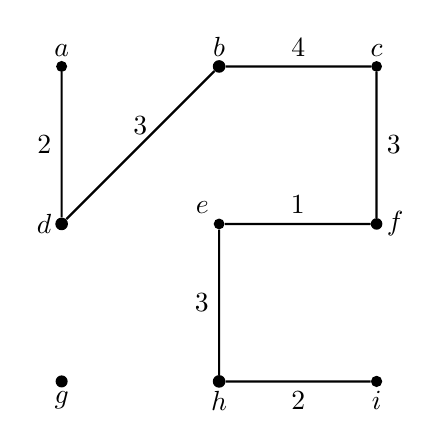
\begin{tikzpicture}[thick]
        \draw (0,0)  node[circle,fill=black,scale=0.25] (a) {a};
        \draw (2,0)  node[circle,fill=black,scale=0.25] (b) {b};
        \draw (4,0)  node[circle,fill=black,scale=0.25] (c) {c};
        \draw (0,-2) node[circle,fill=black,scale=0.25] (d) {d};
        \draw (2,-2) node[circle,fill=black,scale=0.25] (e) {e};
        \draw (4,-2) node[circle,fill=black,scale=0.25] (f) {f};
        \draw (0,-4) node[circle,fill=black,scale=0.25] (g) {g};
        \draw (2,-4) node[circle,fill=black,scale=0.25] (h) {h};
        \draw (4,-4) node[circle,fill=black,scale=0.25] (i) {i};
        \node[above] at (0,0) {$a$};
        \node[above] at (2,0) {$b$};
        \node[above] at (4,0) {$c$};
        \node[left] at (0,-2) {$d$};
        \node[above left] at (2,-2) {$e$};
        \node[right] at (4,-2) {$f$};
        \node[below] at (0,-4) {$g$};
        \node[below] at (2,-4) {$h$};
        \node[below] at (4,-4) {$i$};
        \draw (a) -- (d) node [midway, left] {2}
              (b) -- (d) node [midway, above] {3}
              (b) -- (c) node [midway, above] {4}
              (c) -- (f) node [midway, right] {3}
              (e) -- (f) node [midway, above] {1}
              (e) -- (h) node [midway, left] {3}
              (h) -- (i) node [midway, below] {2};
    \end{tikzpicture}
    \end{figure*}
    \newline and then $h \rightarrow g$ with weight 4
    \begin{figure*}[!htbp]
        \centering
    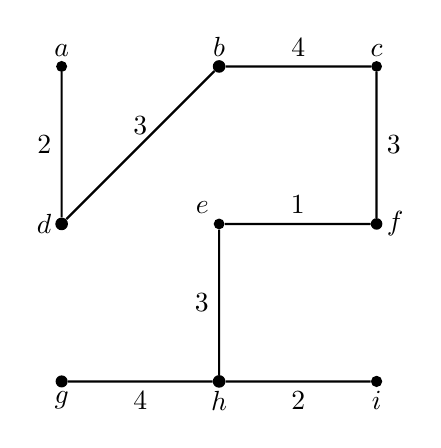
\begin{tikzpicture}[thick]
        \draw (0,0)  node[circle,fill=black,scale=0.25] (a) {a};
        \draw (2,0)  node[circle,fill=black,scale=0.25] (b) {b};
        \draw (4,0)  node[circle,fill=black,scale=0.25] (c) {c};
        \draw (0,-2) node[circle,fill=black,scale=0.25] (d) {d};
        \draw (2,-2) node[circle,fill=black,scale=0.25] (e) {e};
        \draw (4,-2) node[circle,fill=black,scale=0.25] (f) {f};
        \draw (0,-4) node[circle,fill=black,scale=0.25] (g) {g};
        \draw (2,-4) node[circle,fill=black,scale=0.25] (h) {h};
        \draw (4,-4) node[circle,fill=black,scale=0.25] (i) {i};
        \node[above] at (0,0) {$a$};
        \node[above] at (2,0) {$b$};
        \node[above] at (4,0) {$c$};
        \node[left] at (0,-2) {$d$};
        \node[above left] at (2,-2) {$e$};
        \node[right] at (4,-2) {$f$};
        \node[below] at (0,-4) {$g$};
        \node[below] at (2,-4) {$h$};
        \node[below] at (4,-4) {$i$};
        \draw (a) -- (d) node [midway, left] {2}
              (b) -- (d) node [midway, above] {3}
              (b) -- (c) node [midway, above] {4}
              (c) -- (f) node [midway, right] {3}
              (e) -- (f) node [midway, above] {1}
              (e) -- (h) node [midway, left] {3}
              (h) -- (i) node [midway, below] {2}
              (h) -- (g) node [midway, below] {4};
    \end{tikzpicture}
    \end{figure*}
    \newline since there is no vertex left, we get the minimum spanning tree.
\end{solution}

\end{document}